\section{Android Sound Stack}
In this section we describe the Android sound stack.
First we will go through the stack and briefly describe the different parts.
Then we focus on the parts of the stack which is relevant for us.
%Noget indledende tekst forklarende hvorfor vi ser på Android sound stacken
%Noget overblik over sektionen

\subsection{The Sound Stack}
The Android sound stack is all the different components which makes up the sound system on Android devices.
The focus is the audio part of Android, so only audio related \acp{API} and systems will be mentioned at each step. 
On \cref{fig:sound_stack} the full sound stack can be seen.

\paragraph{Application Framework}
On the top of the stack is the application framework.
The frameworks an app, coded in Java, use when dealing with sound is a part of the application framework,
for instance the \code{android.media.*} frameworks.
The application framework is important to consider if the app is made in Java,
since it is the only thing the Java app interfaces with directly.%maybe better argument

\paragraph{JNI}
Below the Application Framework is the \ac{JNI}.
The \ac{JNI} makes it possible for Java code to call and be called by the native applications\cite{jni}.

\paragraph{Native Framework}
The native framework is below the \ac{JNI} and used for implementing apps which runs natively on the system.
To run natively on the system the app can be written in C++.

Using the native framework can give improved performance compared to the application framework used with Java\cite{nat_perf_2}.
This can result in lower latency, and could potential be an advantage when dealing with synchronization of audio.
Therefore the native framework should be considered when designing an app to solve the problem statement.

\paragraph{Binder IPC Proxies}
Below the Native Framework is the Binder IPC Proxies.
The purpose of the Binder IPC Proxies is to facilitate communication over process boundaries.

\paragraph{Media Server}
Below the Binder ICP Proxies, but on \cref{fig:sound_stack} right of the native framework, is the media server.
The Media Server contains the audio services, which is the code that interacts with the \ac{HAL} layer,
right below the Media Server, in the sound stack.
The sound server implementation on Android is called AudioFlinger, and runs within the media server process\cite{audioflinger}.

It is possible to change the media server, 
for instance examples are given where changing from AudioFlinger saved $8 ms$ on the round--trip latency on a HTC Nexus 9\cite{superpowered_8ms}.
The round--trip latency is the time it takes sound to be recorded by the microphone,
travel through the audio stack to the user application and then back through the stack to the speakers\cite{superpowered_8ms}.
Since audio latency can be saved by making changes to the media server,
then it should be taken into account when designing an app to solve the problem statement.

\paragraph{Hardware Abstraction Layer}
Below the Media Server is the \ac{HAL}.
The \ac{HAL} is the standard interface between the audio services and the audio hardware.
The \ac{HAL} is driver--agnostic, which means it can work with any drivers without making any special adaptations.

\paragraph{Linux Kernel}
At the bottom of the stack is the Linux Kernel.
In the Linux Kernel is the audio driver is residing,
there exists different audio drivers, e.g. \ac{ALSA}, \ac{OSS} or custom drivers. 

\begin{figure}[!bht]
    \centering
    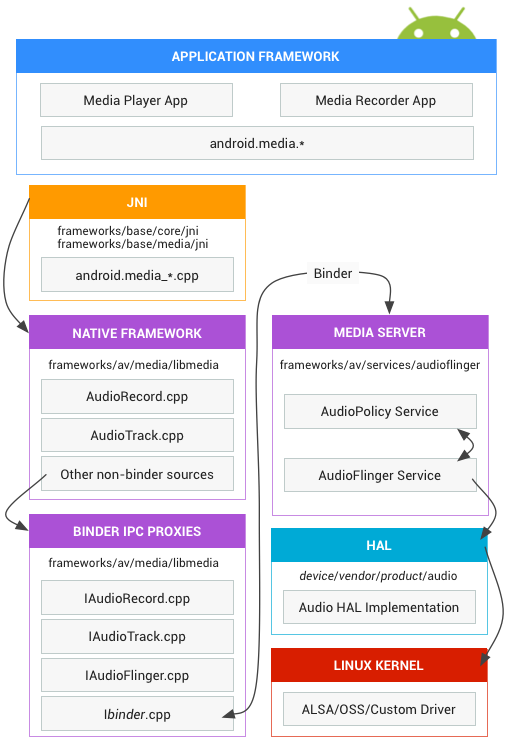
\includegraphics[width=0.5\textwidth]{img/sound_stack.png}
    \caption{The Android audio stack\cite{sound_stack}.}
    \label{fig:sound_stack}
\end{figure}

\subsection{Application Framework}
\subsection{Native Framework}
\subsection{Media Server}
\subsection{Linux Kernel}
\subsection{Summary}
%Hvad fandt vi ud af.

%https://source.android.com/devices/audio/index.html Main source, dog skal mange af de enkelte punkter findes mere dybdegående information om andetsteds. 
%http://androidsexample.blogspot.dk/2015/01/android-audio-architecture.html Kun som inspiration til en TikZ figur
%https://source.android.com/devices/

